\documentclass[10pt]{beamer}

\usetheme{CambridgeUS}
\usepackage[english, russian]{babel}
\usepackage[utf8]{inputenc}
\usepackage{caption}
\usepackage{etoolbox}
\usepackage{multicol}
\AtBeginEnvironment{minted}{\singlespacing%
    \fontsize{10}{10}\selectfont}

\title[\href{https://goo.gl/NRgp8K}{https://goo.gl/NRgp8K} (Term 3)]{Применения суффиксных структур}
\author[Гусев Илья]{Гусев Илья}
\institute[МФТИ] 
{Московский физико-технический институт\\*}
\date{Москва, 2018}
\subject{Computer Science}

\begin{document}

\begin{frame}
  \titlepage
\end{frame}

\begin{frame}{Содержание}
\tableofcontents
\end{frame}

\section{Нахождение числа уникальных подстрок}
\begin{frame}[fragile]{Нахождение числа уникальных подстрок}
\begin{enumerate}
    \item Построение суфф. массива
    \item Построение массива LCP
\end{enumerate}
$$\sum_{i=0}^{n-1} |S_{Suf[i]}| - LCP[i]$$
\end{frame}

\section{Наибольшая общая подстрока K строчек}
\begin{frame}[fragile]{Наибольшая общая подстрока K строчек}{Суфф. массив}
\begin{enumerate}
    \item Построение суфф. массива для $concat(S^1, \$^1 \dots S^k, \$^k)$
    \item Построение массива LCP
    \item Поддерживаем окошко от i до j (индексы в суфф.массе), в котором встретились подстроки из всех K строк
    \item Минимум LCP на этом окошке - общая подстрока K строк
    \item Окошко двигаем, меняем максимум
    \item Сложность?
\end{enumerate}
\end{frame}

\begin{frame}[fragile]{Наибольшая общая подстрока K строчек}{Суфф. массив}
\begin{enumerate}
    \item Построение суфф. массива для $concat(S^1, \$^1 \dots S^k, \$^k)$
    \item Построение массива LCP
    \item Поддерживаем окошко от i до j (индексы в суфф.массе), в котором встретились подстроки из всех K строк
    \item Минимум LCP на этом окошке - общая подстрока K строк
    \item Окошко двигаем, меняем максимум
    \item Сложность: $O(n \cdot log(n))$ или $O(n)$ на построение суфф. массива, $O(n)$ на Касаи, $O(n)$ на основную часть
\end{enumerate}
\end{frame}

\begin{frame}[fragile]{Наибольшая общая подстрока K строчек}{Суфф. дерево}
\begin{enumerate}
    \item Построение обобщённого суфф. дерева для K строк
    \item Для внутренних вершин пишем, откуда мы в них приходили. Например, если мы в нееё дошли из 1, 2, 3 строки, пишем \{1, 2, 3\}
    \item Наиболее глубокая вершина с $\{1, \dots, k\}$ - ответ
    \item Сложность?
\end{enumerate}
\end{frame}

\begin{frame}[fragile]{Наибольшая общая подстрока K строчек}{Суфф. дерево}
\begin{enumerate}
    \item Построение обобщённого суфф. дерева для K строк
    \item Для внутренних вершин пишем, откуда мы в них приходили. Например, если мы в нееё дошли из 1, 2, 3 строки, пишем \{1, 2, 3\}
    \item Наиболее глубокая вершина с \{1, \dots, K\} - ответ
    \item Сложность:$O(n)$ на Укконена, $O(n \cdot K)$ на основную часть. Можно ли за $O(n)$? Можно!
\end{enumerate}
\end{frame}

\begin{frame}[fragile]{Наибольшая общая подстрока K строчек}{Суфф. дерево}
\begin{enumerate}
    \item Построение обобщённого суфф. дерева для K строк
    \item Нам достаточно количества уникальных встреч со строками $S^1 \dots S^k$!
    \item Можем посчитать количество листьев в любом поддереве за O(n) Обозначим за $S(v)$ количество листьев в поддереве вершины v
    \item Можем посчитать количество 'дубликатов' для i-ой строки в любом поддереве за O(n)! Обозначим это за U(v)
    \item Для каждой вершины узнаём C(v) = S(v) - U(v). Где C(v) == k и наибольшая глубина - наш ответ
    \item Сложность: $O(n)$
\end{enumerate}
\end{frame}

\begin{frame}[fragile]{Наибольшая общая подстрока K строчек}{Суфф. дерево}
Считаем количество 'дубликатов' для i-ой строки в любом поддереве за O(n).
\begin{enumerate}
    \item DFS, запоминаем номера суффиксов i-ой строки
    \item Считаем LCA для соседних номеров в получившихся массивах
    \item Для каждой вершины, считаем сколько раз мы считали LCA в поддереве
    \item Это и есть U(v)
\end{enumerate}
\begin{center}
    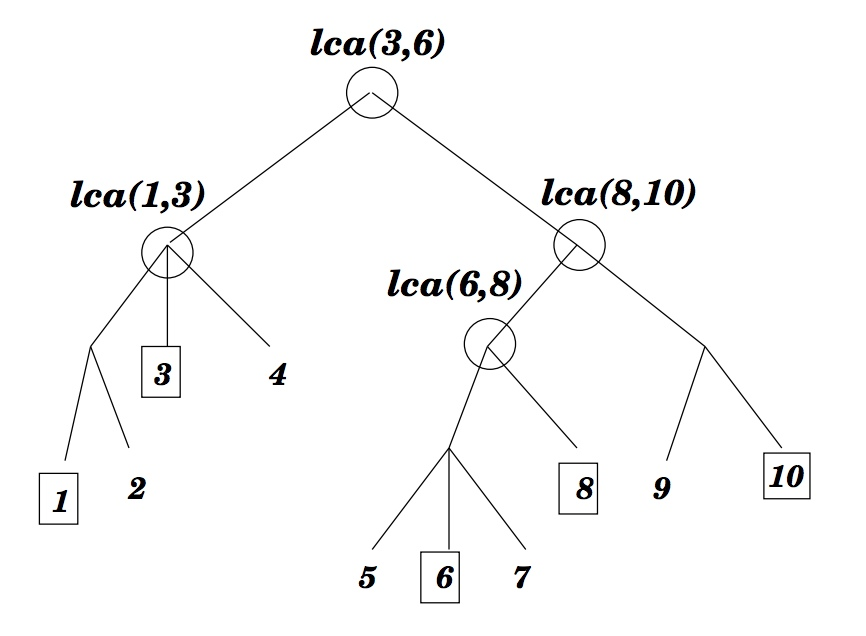
\includegraphics[width=6cm, height=4cm]{Term_3/Source/Pictures/Uv.jpg}
\end{center}
\end{frame}

\section{Наибольшая подстрока-палиндром}
\begin{frame}[fragile]{Наибольшая подстрока-палиндром}{Суфф. массив}
\begin{enumerate}
    \item $SR = s_1 \dots s_n \# s_n \dots s_1 \$$
    \item Построение суфф. массива
    \item Построение LCP
    \item Идеём последовательно по массиву
    \begin{itemize}
        \item Если левый суффикс из прямой строки, а правый из обратной (или наоборот), то это нам подходит.
        \item Кроме того, проверяем, что суффикс обратной строки захватывает суффикс прямой (их пересечение непустое, lcp + s + r = len(S))
        \item Берём максимум из LCP таких пар
    \end{itemize} 
\end{enumerate}
\end{frame}

\begin{frame}[fragile]{Наибольшая подстрока-палиндром}{Суфф. дерево}
\begin{enumerate}
    \item $S = s_1 \dots s_n \#$
    \item $S^T = s_n \dots s_1 \$$
    \item Рассматриваем $S_i$ и $S^T_{n-i+1}$
    \item Ищем их LCA, смотрим на его глубину
    \item Повтрояем для всех i, берём вершину с наибольшей глубиной
    \item Достраиваем её до палиндрома в зависимости от чётности
\end{enumerate}
\begin{center}
    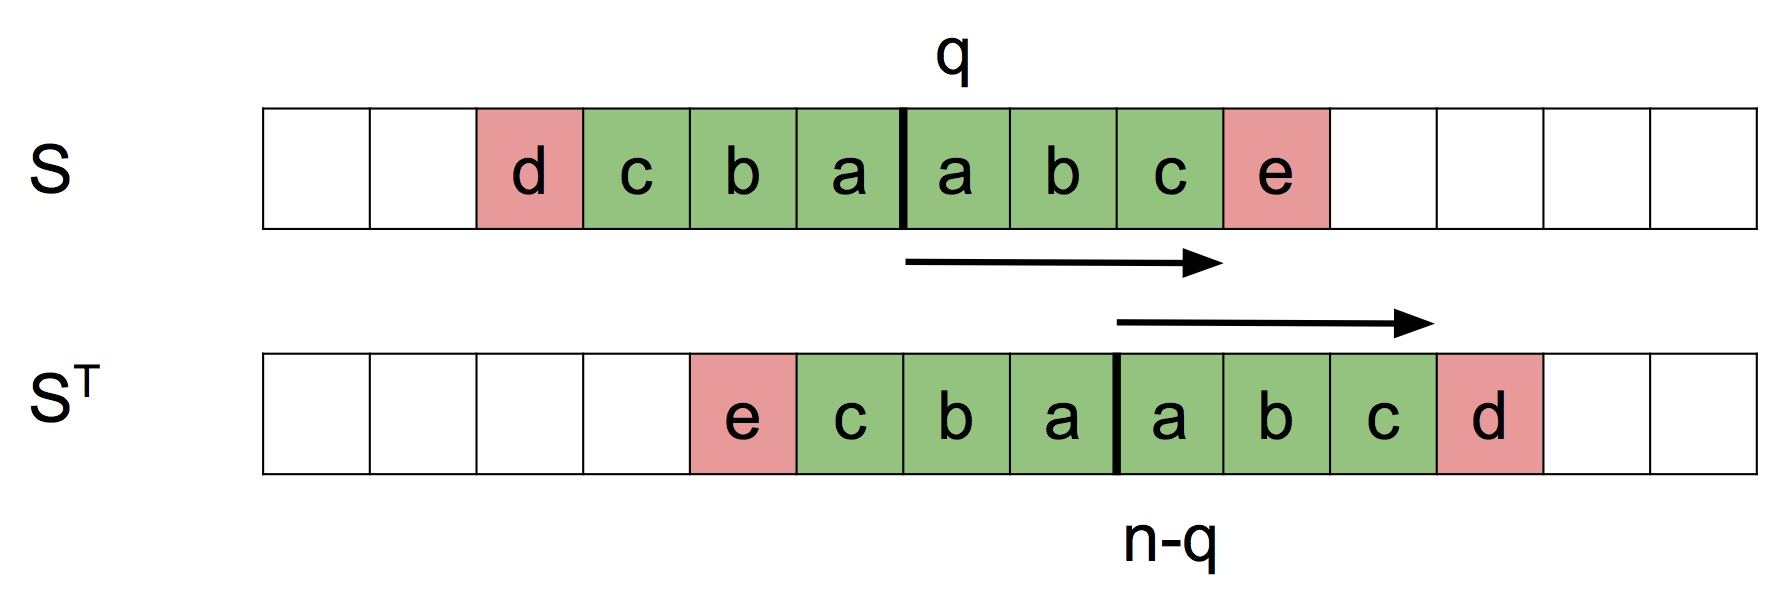
\includegraphics[width=12cm, height=4cm]{Term_3/Source/Pictures/pal.jpg}
\end{center}
\end{frame}

\section{Поиск количества непересекающихся вхождений строки в текст}
\begin{frame}[fragile]{Поиск количества непересекающихся вхождений строки в текст}{Суфф. массив}
\begin{itemize}
    \item Построение суфф. массива
    \item Построение LCP
    \item Поиск вхождений строки в текст (непрерывный диапазон в суффиксном массиве)
    \item Сортировка этого диапазона по оригинальному номеру суффикса
    \item Магия индексов
\end{itemize}
\end{frame}

\appendix
\section<presentation>*{\appendixname}
\subsection<presentation>*{Useful links}

\begin{frame}[allowframebreaks]
  \frametitle<presentation>{Полезные ссылки}
    
  \begin{thebibliography}{10}
{
  \beamertemplatebookbibitems
  % Start with overview books.
  
  \bibitem{apl}
  \texttt{APL6: Common substrings of more than two
strings}
  \newblock \href{http://web.cs.ucdavis.edu/\~gusfield/cs224f11/commonsubstrings.pdf}{\texttt{http://web.cs.ucdavis.edu/\~gusfield/cs224f11/commonsubstrings.pdf}}
  
  \bibitem{so1}
  \texttt{SO: Longest palindrome in a string using suffix tree}
  \newblock \href{https://bit.ly/2A7Q5BX}{\texttt{https://bit.ly/2A7Q5BX}}
  
    \bibitem{quora1}
  \texttt{Quora: How can I find the longest common substring of three or more strings using a suffix array?}
  \newblock \href{https://bit.ly/2yz80PX}{\texttt{https://bit.ly/2yz80PX}}
}
    
  \end{thebibliography}
\end{frame}

\end{document}


